\documentclass[10pt]{article}
\usepackage[margin=0.5in]{geometry}
\usepackage{hyperref}
\usepackage{xcolor}
\usepackage{lmodern}
\usepackage{microtype}
\usepackage{tikz}
\usetikzlibrary{arrows.meta,positioning,shapes.geometric,fit}

\hypersetup{colorlinks=true, linkcolor=blue, urlcolor=blue, citecolor=blue}

\makeatletter
\renewcommand{\section}{\@startsection{section}{1}{0pt}{0.4ex plus 0.1ex}{0.15ex}{\normalfont\bfseries}}
\makeatother

\setlength{\parskip}{0.15em}
\setlength{\parindent}{0em}
\pagestyle{empty}
\sloppy

\begin{document}

\begin{center}
{\bfseries DMREF Concept Outline --- Critical-Mineral-Lean Printable Aluminum Alloys via CALPHAD--BOFN Discovery and Ultrasonic Atomization}
\end{center}

{\small \textbf{PI:} Sterling Baird (Brigham Young University, Materials Science \& Engineering). \textbf{Solicitation:} NSF DMREF (NSF~25-508). \textbf{Type:} 4-yr, multi-PI, $\sim$\$1.5--2.0M. \textbf{Anticipated cycle:} Jan--Feb~2027. \textbf{Keywords:} MGI, BOFN, CALPHAD, LPBF, ultrasonic atomization, critical materials.}

% Shared FLAIME pipeline DAG used by all three concept outlines.
% Requires \usepackage{tikz} and \usetikzlibrary{arrows.meta,positioning,shapes.geometric,fit}
\begin{center}
\resizebox{\textwidth}{!}{%
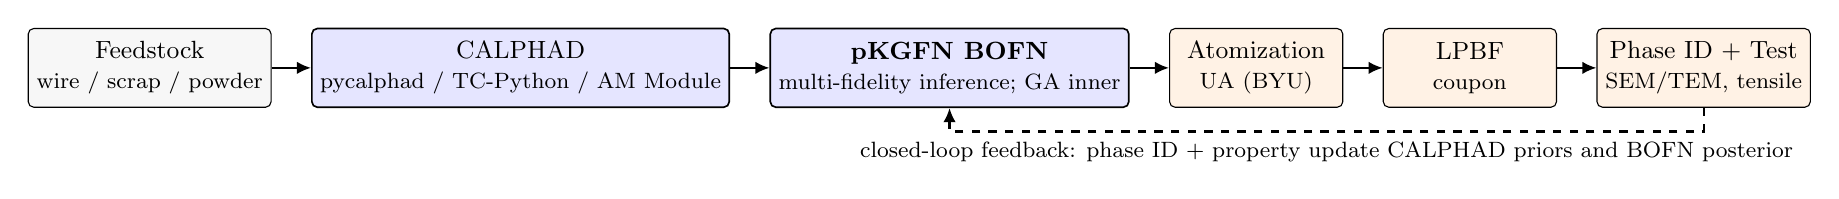
\begin{tikzpicture}[
    node distance=4.5mm and 5mm,
    every node/.style={font=\small},
    block/.style={rectangle, draw, rounded corners=2pt, align=center,
                  minimum height=10mm, minimum width=22mm, inner sep=3pt,
                  fill=black!3},
    ai/.style={block, fill=blue!10, line width=0.6pt},
    expt/.style={block, fill=orange!10},
    arr/.style={-{Latex[length=1.8mm,width=1.6mm]}, thick}
]
  \node[ai] (cal) {CALPHAD\\\footnotesize{pycalphad / TC-Python / AM~Module}};
  \node[ai, right=of cal] (bofn) {\bfseries pKGFN BOFN\\\footnotesize{multi-fidelity inference; GA inner}};
  \node[block, left=of cal] (feed) {Feedstock\\\footnotesize{wire / scrap / powder}};
  \node[expt, right=of bofn] (ua) {Atomization\\\footnotesize{UA (BYU)}};
  \node[expt, right=of ua] (lpbf) {LPBF\\\footnotesize{coupon}};
  \node[expt, right=of lpbf] (test) {Phase ID + Test\\\footnotesize{SEM/TEM, tensile}};
  \draw[arr] (feed) -- (cal);
  \draw[arr] (cal) -- (bofn);
  \draw[arr] (bofn) -- (ua);
  \draw[arr] (ua) -- (lpbf);
  \draw[arr] (lpbf) -- (test);
  % Loop-closure feedback arrow under the row.
  \draw[arr, dashed] (test.south) -- ++(0,-3mm) -| node[below, pos=0.25, font=\footnotesize]
      {closed-loop feedback: phase ID + property update CALPHAD priors and BOFN posterior} (bofn.south);
\end{tikzpicture}%
}
\end{center}


\section*{Fundamental question}
What controls the printability and elevated-temperature phase stability of dilute multi-principal-element Al alloys built from Mn/Cr/Zr/Si/Fe additions, in the regime where conventional CALPHAD assessments are sparse and rapid-solidification AM thermal histories drive non-equilibrium phase selection? The MGI-relevant gap is not optimization of an existing alloy family but predictive thermodynamic understanding of a region of Al-MPEA phase space that has been opaque because the validation pipeline (CALPHAD $\to$ atomization $\to$ AM $\to$ phase ID) has never been closed end-to-end.

\section*{Idea}
A 4-yr DMREF project using a single joint pKGFN BOFN acquisition over a constrained Al-MPEA design space (Al + dilute Mn/Cr/Zr/Si/Fe, $\le$6 active solute elements, with the remaining critical-materials-relevant elements held at zero unless evidence supports activation), with CALPHAD multi-fidelity nodes (\texttt{pycalphad}, TC-Python/TCAL10, Thermo-Calc AM~Module) as parallel partial-evaluation/context nodes. UA + LPBF serve as the experimental validation tier; their parameters are nuisance variables, not design targets. \textbf{Hypothesis:} the rapid-solidification phase fields accessible via UA + LPBF in dilute Al-Mn-Cr-Zr-Si space contain metastable strengthening phases that are absent from current CALPHAD databases and that can be predicted by a closed BOFN--CALPHAD--experiment loop. The scientific deliverable is a measured, openly published correction to the Al-MPEA phase diagram in this regime, with the BOFN--CALPHAD loop as the methodological tool. Composition/process/property records are deposited to the Materials Data Facility with cradle-to-coupon provenance.

\section*{Why DMREF (MGI fit, multi-PI structure)}
\emph{MGI alignment:} closed-loop computation $+$ experiment $+$ open data targeting fundamental thermodynamics, not parameter tuning of a known alloy. \emph{Multi-PI structure (NSF-fundable):} BYU (Baird, lead --- BOFN, CALPHAD, phase ID, tensile). \emph{Unfunded U.S. collaborator:} U.~Utah (Spear lab --- no-cost LPBF coupon access via established MOU; not a subaward). \emph{Unfunded international collaborator:} U.~Toronto (J.~Hattrick-Simpers, Acceleration Consortium --- autonomous-experimentation methods cross-validation; supported through separate NSERC funds, not via NSF subaward). \emph{Unfunded national-lab collaborator:} CMI Hub at Ames (existing letter; supply-risk context only; per DMREF rules Ames brings its own DOE funding). \emph{Industrial collaborator:} Thermo-Calc (CALPHAD database access).

\section*{Preliminary results (FLAIME pipeline, BYU, Apr~2026) and Y1 scientific milestone}
AMAZEMET rePOWDER UA atomizer installed and operational; UA composition modification from AlSi10Mg + Al wire + Si feed confirmed by SEM/EDS (the wire-to-powder pathway is in working form). AlSi10Mg LPBF tensile coupon printed at U.~Utah (Spear lab); elevated-temperature tensile data on a standard Al specimen. Working pKGFN BOFN implementation; Thermo-Calc AM~Module simulations on candidate FLAIME compositions; CALPHAD jobs on BYU HPC. \emph{Y1 scientific milestone (the prediction-validation example DMREF reviewers should expect):} one closed-loop case in which the BOFN--CALPHAD posterior predicts a metastable phase in a defined Al-Mn-Cr-Zr-Si window that the public Al-database equilibrium assessment ranks differently, with SEM/TEM phase ID on a UA + LPBF coupon to confirm or refute the prediction.

\section*{Scope separation from pending DOE Genesis Mission Topic~3B}
The two efforts are separated at the task and deliverable level, not just by narrative. \emph{Genesis tasks (DOE-funded):} hardware/software integration of an autonomous LPBF-AM platform; scheduler; data fabric; alloy-agnostic platform validation. \emph{DMREF tasks (NSF-funded):} (T1)~hypothesis-driven CALPHAD-BOFN study of non-equilibrium phase selection in dilute Al-Mn-Cr-Zr-Si space; (T2)~thermodynamic-database correction in that regime; (T3)~open scientific data products (MDF deposition, CALPHAD overlay files). Personnel effort, deliverables, and reporting artifacts are itemized separately; no budget line, equipment purchase, or scheduler-development task appears in both. Current-and-pending will reflect this split explicitly.

\section*{Request}
A brief read on whether this concept appears potentially responsive to DMREF and whether a short scoping call would be useful before BYU's internal limited-submission process for the Jan--Feb~2027 window.

{\small \emph{Repository and full vision:} \url{https://github.com/vertical-cloud-lab}.}

\end{document}
